
Data is transmitted everywhere in the air around us. As the data demand gets larger each year, engineers make use of all of the different 
channels and bands. People these days discover that the transmission channels are in fact limited. In many countries, there is an administrative
agency which regulates the band allocation. Here in United States, the National Telecommunications and Information Administration 
(NTIA) and the Federal Communications Commission (FCC) are responsible for allocating bands for government, organizational and
individual uses. A licensed band user is given a range of frequency in the spectrum where they can freely utilize data transmission
in the air. However, recent studies report, at certain frequencies (bands), there is only a low 15 percent of utilization, where other
channels were overwhelming with data crossing. This creates large load distribution gaps as shown in Figure~\ref{fig:spectrum_utilization}.

\begin{figure}[ht]
\centering
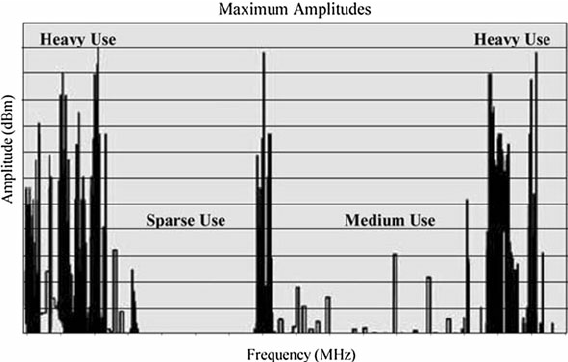
\includegraphics[width=12cm]{figures/spectrum_utilization.png}
\caption{Spectrum Utilization \cite{improved_local}}
\label{fig:spectrum_utilization}
\end{figure}

It is possible to balance the load across the whole spectrum. By keeping this objective in mind, scientists have proposed spectrum 
management solutions year to year; one of these solutions is using Cognitive Radio (CR). CR is under the category of Software Defined Radio 
(SDR), which is programmable and adaptive to varying complex environment \cite{software_defined_radio}. Regarding the topic of Cognitive Radio Network (CRN), it is still a broad, ongoing research project. One area that people research for is optimizing the channel utilization. They generally looking for the best channel handoff algorithm to avoid more "holes" in the channel shown in Figure~\ref{fig:channel_hole}. A good handoff algorithm can fill in much of the holes during the transmission process. This directly improve the spectrum utilization. Many related papers claim to have a 
more efficient algorithm compared to others, more specifically, they are looking at the effects of different channel 
selection algorithms. A two phase real-time spectrum handoff algorithm that Chakraborty and Misra propose in their conference paper confirms a 40 to 60 percent decrease in spectrum handoff delay in simulation models \cite{real_time_spectrum}. Analytically, it has a minimum 10 percent reduction in Voice over IP (VoIP) call-dropping probability. In Varade and Ravinder's paper, in simulation, they show their Genetic Algorithm (GA) resulting a overall efficiency of 94 percent of fitness measures by optimizing transmission parameters \cite{optimal_spectrum_allocation}.

\begin{figure}[ht]
\centering
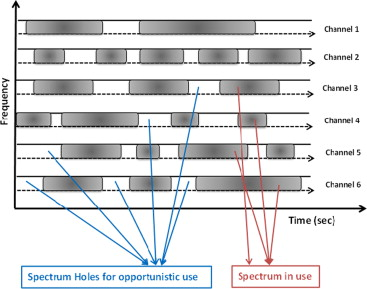
\includegraphics[width=12cm]{figures/channel_hole.jpg}
\caption{Spectrum Utilization \cite{idle_channel}}
\label{fig:channel_hole}
\end{figure}

This thesis project contributes to the field by compiling an emulator that composes scalable software integration and accessible
hardware for the CRN. Notice not many paper under the area actually deploy hardware to test their program for the network 
With all those intelligent channel selection algorithms from proposers, testing them at real time should essentially be the 
next step. Yet, they hesitate to move forward, one reason is because we do expect a significant spending on the setup of the physical 
testing environment. Before the full development of a specific hardware for systematic testing are put into action, a general purposed testbed 
can make it easier to validate any functional characteristic with proposed algorithm. 
A desire physical testbed can adapt to different program and stimulus. Ultimately, it records and return meaningful data that entail the performance of the system under test.

Using the thesis project emulator framework for real time experiment, to a good extent, one can estimate the performance of a channel 
selection algorithm. It costs well under \$50 for the whole system. If experiment run time is an issue, one can adjust
the timing ratio to minimize the uses of resource. Despite of its simplicity, the implementation follows closely to IEEE
standard and FCC guildline.

To understand the significant of the project, the thesis paper first explains some of the background of the technology in Chapter 2.
Chapter 3 describes the design choices during software development. Chapter 4 illustrates physical modules and a fine prototype.
To test the usability of the system, the project included a performance comparison of a channel selection method with history table and in-order/random selection in Chapter 5. Last chapter, Chapter 6 concludes the work and discuss its future possible route. 



